\section{Introduction}

This article attempts to answer the following questions.

\begin{itemize}
\item I know how to derive the equations of motion for one rigid body
  and I have seen people use the following equations for articulated
  rigid bodies, but I don't know how they are derived?
\begin{equation}
M(\vc{q}) \ddot{\vc{q}} + C(\vc{q}, \dot{\vc{q}})  = \vc{Q} \nonumber
\end{equation}

\item I have seen Lagrangian equation in the following form before, but I
  don't know how it is related to the equations of motion above.
\begin{equation}\label{eq:lagrangian_dyn}
    \frac{d}{dt} \left( \frac{\partial \sKinetics_i}{\partial
    \dot{\vJoint}} \right) - \frac{\partial \sKinetics_i}{\partial
    \vJoint} - \vc{Q} = 0 \nonumber
\end{equation}

\item I use generalized coordinates to compute the control forces, how do I convert them to Cartesian forces such that I can use simulators like ODE, PhysX, or Bullet which represent rigid bodies in the maximal coordinates?
\item I heard of Featherstone algorithm. What is it and how is it related to Lagrangian dynamics?
\end{itemize}

\section{Lagrangian Dynamics}
\label{sec:lagrangian}
Articulated human motions can be described by a set of dynamic
equations of motion of multibody systems. Since the direct
application of Newton's second law becomes difficult when a
complex human skeleton is considered, we use \emph{Lagrange's
equations} derived from \emph{D'Alembert's principle} to describe
the dynamic of the motions. The entire human skeleton is consist
of a collection of particles $\{\vGlobalPoint_1, \vGlobalPoint_2,
\ldots, \vGlobalPoint_{\sNumParticle}\}$.  Each particle,
$\vGlobalPoint_i$, is defined by Cartesian coordinates that
describe the translation with respective to the world coordinates.
We can represent $\vGlobalPoint_i$ by a set of \emph{generalized
coordinates} that indicate the joint configuration of the human
skeleton:

\begin{equation}\label{eq:general_coord}
    \vGlobalPoint_i = \vGlobalPoint_i(\sJoint_{1},
\sJoint_{2}, \ldots, \sJoint_{\sNumJoint}, t)
\end{equation}
where $t$ is the time and $\sJoint_j$ is a joint angle value in
the skeleton.

The virtual displacement $\delta \vGlobalPoint_i$ refers to an
infinitesimal change in the system coordinates such that the
constraint remains satisfied. In the context of human skeleton, the
system coordinates are the generalized coordinates $\sJoint_j$ and the
constraint manifold lies in the Cartesian space. The virtual
displacement $\delta \vGlobalPoint_i$ is a tangent vector to the
constraint manifold at a fixed time, written as

\begin{equation}\label{eq:virtual_displace}
    \delta \vGlobalPoint_i = \sum_j \frac{\partial \vGlobalPoint_i}{\partial
    \sJoint_j}\delta \sJoint_j
\end{equation}

We can write virtual work of force $\vForce{i}$ acting on particle
$\vGlobalPoint_i$ as
\begin{equation}\label{eq:virtual_work}
  \vForce{i} \delta \vGlobalPoint_i = \vForce{i} \sum_j \frac{\partial \vGlobalPoint_i}{\partial
    \sJoint_j}\delta \sJoint_j = \sum_j \sGeneralForce{j} \delta \sJoint_j
\end{equation}
where $\sGeneralForce{j}$ is defined as \emph{generalized force}
associated with coordinate $\sJoint_j$.

From D'Alembert's principle, we know that the sum of the differences
between the forces acting on a system and the inertia force of the
system along any virtual displacement consistent with the constraints
of the system, is zero. Therefore, the virtual work at $\vGlobalPoint_i$ can be written as
\begin{equation}\label{eq:inertial_work}
  \delta \sWork_i = \vForce{i} \delta \vGlobalPoint_i = \sInfMass_i \ddot{\vGlobalPoint}_i \cdot
    \delta \vGlobalPoint_i = \sum_j \sInfMass_i \ddot{\vGlobalPoint}_i \cdot
    \frac{\partial \vGlobalPoint_i}{\partial \sJoint_j} \delta \sJoint_j
\end{equation}
where $\sInfMass_i$ is the infinitesimal mass associated with
$\vGlobalPoint_i$. The component of inertia force associated with
$\sJoint_j$ can be written as
\begin{equation}
\label{eq:inertia_force}
  \sInfMass_i \ddot{\vGlobalPoint}_i \cdot \frac{\partial \vGlobalPoint_i}{\partial \sJoint_j} =
  \frac{d}{dt} \left( \sInfMass_i \dot{\vGlobalPoint}_i \cdot \frac{\partial
  \vGlobalPoint_i}{\partial \sJoint_j} \right) - \sInfMass_i
\dot{\vGlobalPoint}_i \cdot \frac{d}{dt} \left( \frac{\partial
    \vGlobalPoint_i}{\partial \sJoint_j} \right) 
\end{equation}

Now let us consider the velocity of $\vGlobalPoint_i$ in terms of
joint velocity $\dot{\sJoint}_j$
\begin{equation}
\label{eq:velocity}
\dot{\vGlobalPoint}_i = \sum_j \frac{\partial
  \vGlobalPoint_i}{\partial \sJoint_j} \dot{\sJoint}_j
\end{equation}
from which we derive the following two identities:
\begin{eqnarray}
\frac{\partial \dot{\vGlobalPoint}_i}{\partial \dot{\sJoint}_j} &=&
\frac{\partial \vGlobalPoint_i}{\partial \sJoint_j}  \\
\frac{\partial \dot{\vGlobalPoint}_i}{\partial \sJoint_j} &=&
\sum_k \frac{\partial^2 \vGlobalPoint_i}{\partial \sJoint_j \partial
  \sJoint_k} \dot{\sJoint}_k = \frac{d}{dt} \frac{\partial \vGlobalPoint_i}{\partial \sJoint_j}
\end{eqnarray}

Using these two identities, we rewrite Equation \ref{eq:inertia_force} as
\begin{equation}
\label{eq:inertia_force2}
\sInfMass_i \ddot{\vGlobalPoint}_i \cdot \frac{\partial \vGlobalPoint_i}{\partial \sJoint_j}   = \frac{d}{dt} \left[ \frac{\partial}{\partial \dot{\sJoint}_j} \left( \frac{1}{2} \sInfMass_i \dot{\vGlobalPoint}_i^{T} \dot{\vGlobalPoint}_i\right) \right]
   - \frac{\partial}{\partial \sJoint_j} \left( \frac{1}{2} \sInfMass_i \dot{\vGlobalPoint}_i^{T} \dot{\vGlobalPoint}_i \right)
\end{equation}

We can denote the kinetic energy of $\vGlobalPoint_i$ as
\begin{equation}\label{eq:kinetic_energy}
    \sKinetics_i = \frac{1}{2} \sInfMass \dot{\vGlobalPoint}_i^{T}
    \dot{\vGlobalPoint}_i,
\end{equation}
and rewrite Equation \ref{eq:inertia_force2} as
\begin{equation}\label{eq:inertia_kinetic}
    \sInfMass_i \ddot{\vGlobalPoint}_i \cdot \frac{\partial \vGlobalPoint_i}{\partial
    \sJoint_j} = \frac{d}{dt} \left( \frac{\partial \sKinetics_i}{\partial
    \dot{\sJoint}_j}\right) - \frac{\partial \sKinetics_i}{\partial \sJoint_j}
\end{equation}

Combining the definition of generalized force (Equation
\ref{eq:virtual_work}), D'Alembert's principle (Equation
\ref{eq:inertial_work}), and the generalized inertia force (Equation
\ref{eq:inertia_kinetic}), we arrive at the following equation:
\begin{equation}\label{eq:dynamic_equil}
    \left[ \frac{d}{dt} \left( \frac{\partial \sKinetics_i}{\partial \dot{\sJoint}_j} \right) - \frac{\partial \sKinetics_i}{\partial
    \sJoint_j}\right] \delta \sJoint_j = \sGeneralForce{j} \delta
    \sJoint_j
\end{equation}

If the set of generalized coordinates $\sJoint_j$ is linearly
independent, Equation \ref{eq:dynamic_equil} leads to
\emph{Lagrangian equation}:
\begin{equation}\label{eq:lagrangian_dyn}
    \frac{d}{dt} \left( \frac{\partial \sKinetics_i}{\partial
    \dot{\sJoint}_j} \right) - \frac{\partial \sKinetics_i}{\partial
    \sJoint_j} - \sGeneralForce{j} = 0
\end{equation}

\paragraph{Equations of Motion in Vector Form.} Equation
\ref{eq:lagrangian_dyn} is the equation of motion for one generalized coordinate in a
multibody system. We can combine $\sNumJoint$  scalar equations into
the familiar vector form
\begin{equation}\label{eq:lagrangian_vector}
M(\vc{q}) \ddot{\vc{q}} + C(\vc{q}, \dot{\vc{q}}) = \vc{Q} 
\end{equation}
where $M(\vc{q})$ is the mass matrix, $C(\vc{q}, \dot{\vc{q}})$ is the
Coriolis and centrifugal term of the equation of motion, and $\vc{Q}$
is the vector of generalized forces for all the degrees of freedom
(DOFs) in the system. $M$ only depends on $\vc{q}$ and $C$ depends
quadratically on $\dot{\vc{q}}$.

How do we derive $M$ and $C$ from Equation \ref{eq:lagrangian_dyn}?
Let us go back to the velocity of one particle $\vGlobalPoint_i$:
\begin{equation}
\dot{\vGlobalPoint}_i = \sum_j \frac{\partial
  \vGlobalPoint_i}{\partial \sJoint_j} \dot{\sJoint}_j = J_i(\vc{q}) \dot{\vc{q}}
\end{equation}
where $J_i$ denotes the Jacobian of $\vGlobalPoint_i$. By summing up
all the particles in the system, the kinetic
energy of the system can then be expressed as
\begin{equation}
\label{eq:kinetic_vector}
T = \sum_i T_i = \sum_i \frac{1}{2}  \sInfMass \dot{\vGlobalPoint}_i^{T}
    \dot{\vGlobalPoint}_i = \sum_i \frac{1}{2}  \sInfMass (J_i
    \dot{\vc{q}})^T(J_i \dot{\vc{q}}) = \frac{1}{2} \dot{\vc{q}}^T
    (\sum_i \sInfMass J_i^TJ_i) \dot{\vc{q}} = \frac{1}{2}
    \dot{\vc{q}}^T M(\vc{q}) \dot{\vc{q}}
\end{equation}
where we define the mass matrix, $M(\vc{q}) = \sum_i \sInfMass
J_i^TJ_i$, and will shortly show it is indeed the mass matrix in
Equation \ref{eq:lagrangian_vector}.

From Equation \ref{eq:kinetic_vector}, we can derive the derivative
terms to construct the Lagrange's equation (Equation
\ref{eq:lagrangian_dyn}).
\begin{equation}
\frac{d}{dt}\frac{\partial T}{\partial \dot{\vc{q}}} - \frac{\partial
  T}{\partial \vc{q}} = M\ddot{\vc{q}} + \dot{M} \dot{\vc{q}} - \frac{1}{2}\dot{\vc{q}}^T \frac{\partial M}{\partial \vc{q}} \dot{\vc{q}} = M
\ddot{\vc{q}} + C(\vc{q}, \dot{\vc{q}})
\end{equation}
where $C$ is the Coriolis and centrifugal term in Equation
\ref{eq:lagrangian_vector} and is defined as $C = \dot{M}
\dot{\vc{q}} - - \frac{1}{2}\dot{\vc{q}}^T \frac{\partial M}{\partial
  \vc{q}} \dot{\vc{q}}$. Note that the second term of $C$ involves a
tensor multiplication so that $\frac{\partial M}{\partial
  \vc{q}} \dot{\vc{q}}$ is not equivalent to $\dot{M}$.

Once we know how to compute the mass matrix, Coriolis and centrifugal
term, and generalized forces, we can compute the acceleration in
generalized coordinates, $\ddot{\vc{q}}$, for forward
simulation. Conversely, if we are given $\ddot{\vc{q}}$ from a motion
sequence, we can use these equations of motion to derive generalized
forces for inverse dynamics. 

\paragraph{Newton-Euler Equations for a Single Rigid Body.}
\begin{equation}
\left(
\begin{array}{cc}
m\vc{I} & \vc{0} \\
\vc{0} & I_c 
\end{array}
\right)
\left(
\begin{array}{c}
\dot{\vc{v}} \\
\dot{\omega} 
\end{array}
\right) +
\left(
\begin{array}{c}
\vc{0}  \\
\omega \times I_c \omega 
\end{array}
\right) = 
\left(
\begin{array}{c}
\vc{F} \\
\tau 
\end{array}
\right)
\end{equation}
The familiar Newton-Euler equations for a rigid body can be viewed as
a special case of Lagrangian dynamics. We start from writing down the
kinetic energy of the rigid body, whose mass, position of the center
of mass (COM), orientation,
linear velocity, and angular velocity are $m$$, \vc{x}$, $R$,
$\vc{v}$, and $\omega$ respectively (same as defined in Witkin and
Baraff's course notes):

\begin{eqnarray}
\label{eqn:rigid_kinetic}
T &=& \sum_i T_i = \sum_i \frac{1}{2}  \sInfMass \dot{\vGlobalPoint}_i^{T}
    \dot{\vGlobalPoint}_i = \sum_i \frac{1}{2}  \sInfMass (\vc{v} + \omega
    \times \vc{r}_i')^T (\vc{v} + \boldsymbol{\omega}
    \times \vc{r}_i') \nonumber \\
 &=& \sum_i \frac{1}{2}  \sInfMass (\vc{v}^T\vc{v} +
    \vc{v}^T [\omega] \vc{r}_i' + \vc{r}_i'^T [\omega]^T \vc{v} +
    \vc{r}_i'^T [\omega]^T [\omega] \vc{r}_i')
\end{eqnarray}
where $\vc{r}_i' = \vc{r}_i - \vc{x}$. Because $\sum_i \sInfMass
\vc{r}_i' = \vc{0}$, the second term and the third term in Equation
\ref{eqn:rigid_kinetic} vanish. Let us focus on the more interesting
fourth term. Using the identity $[\omega]\vc{r}_i' =
-[\vc{r}_i']\omega$, we can rewrite Equation \ref{eqn:rigid_kinetic}
as:
\begin{equation}
T = \frac{1}{2} m \vc{v}^T\vc{v} - \frac{1}{2} \sum_i \sInfMass
\omega^T [\vc{r}_i'][\vc{r}_i'] \omega
\end{equation}

Recall the inertia tensor defined in Witkin and
Baraff's course notes: $I_c = \sum_i \sInfMass ((\vc{r}_i'^T
\vc{r}_i')\vc{I} - \vc{r}_i' \vc{r}_i'^T)$, where $\vc{I}$ is the
identity matrix. We can easily show that
$I_c = \sum_i -\sInfMass [\vc{r}_i'][\vc{r}_i']$ by verifying the
identity $-[\vc{a}][\vc{a}] = (\vc{a}^T\vc{a}) \vc{I}  -
\vc{a}\vc{a}^T$. As a result, the kinetic energy of a rigid body can
be shown in its vector form:

\begin{eqnarray}
T &=& \frac{1}{2} (\vc{v}^T \;\; \omega^T)
\left(
\begin{array}{cc}
m\vc{I} & \vc{0} \\
\vc{0} & \sum_i -\sInfMass [\vc{r}_i'][\vc{r}_i']
\end{array}
\right)
\left(
\begin{array}{c}
\vc{v} \\
\omega 
\end{array}
\right) \nonumber \\
&=& \frac{1}{2} (\vc{v}^T \;\; \omega^T)
\left(
\begin{array}{cc}
m\vc{I} & \vc{0} \\
\vc{0} & I_c
\end{array}
\right)
\left(
\begin{array}{c}
\vc{v} \\
\omega 
\end{array}
\right)
\end{eqnarray}

Comparing the above equation with Equation
\ref{eq:kinetic_vector}, we define $\dot{\vc{q}}^T = (\vc{v}^T \;\;
\omega^T)$ and mass matrix $M(\vc{q}) =
\left(\begin{array}{cc}m\vc{I} & \vc{0} \\ \vc{0} &
    I_c \end{array}\right)$. Let us now compute the Coriolis and
centrifugal term $C = \dot{M}
\dot{\vc{q}} - \frac{1}{2}\dot{\vc{q}}^T \frac{\partial M}{\partial
  \vc{q}} \dot{\vc{q}}$. The first term is computed as
\begin{eqnarray}
\label{eqn:mdotqdot}
\dot{M}\dot{\vc{q}} &=& \left(\begin{array}{cc}
\vc{0} & \vc{0} \\ 
\vc{0} &   \dot{I}_c 
\end{array}\right)
\left(\begin{array}{c}\vc{v} \\ \omega\end{array}\right) = 
\left(\begin{array}{c}\vc{0} \\ \dot{I}_c \omega\end{array}\right)
\nonumber \\
& = & \left(\begin{array}{c}\vc{0} \\ \dot{(R I_b R^T)}
    \omega\end{array}\right) = \left(\begin{array}{c}\vc{0} \\ \dot{R}
    I_b R^T \omega + R I_b \dot{R}^T \omega \end{array}\right)
\nonumber \\
& = & \left(\begin{array}{c}\vc{0} \\ \;[\omega] R I_b R^T \omega + R
    I_b R^T [\omega]^T \omega \end{array}\right) =
\left(\begin{array}{c}\vc{0} \\ \;[\omega] I_c \omega - I_c\omega \times \omega \end{array}\right) \nonumber \\
& = & \left(\begin{array}{c}\vc{0} \\ \omega \times I_c \omega \end{array}\right)
\end{eqnarray}
where $I_b$ is the inertia tensor defined in the local frame. The
third line in Equation \ref{eqn:mdotqdot} uses the relation of angular
velocity $\dot{R} = [\omega] R$ and the skew symmetric property
$[\omega]^T = -[\omega]$.

The second term of the Coriolis and centrifugal term involves tensor
multiplication due to the term $\frac{\partial M}{\partial
  \vc{q}}$. We will demonstrate how it is computed using only one
element of $\vc{q}$ for clarity. \karen{ Hmm, in my derivation this
  term turns out to be -$\omega \times I_c \omega $ while I
  expect it to be 0. Where
  could it go wrong?}


\section{Conversion between Cartesian and Generalized Coordinates}
In practice, we often want to use third-party rigid body simulators
rather than develop our own. There are a few widely used physics
engines that provide efficient, robust, and fairly accurate rigid body
simulation and collision handling. Open Dynamic Engine (ODE), PhysX, and
Bullet are perhaps the most popular free choices among game developers and
academic researchers. These commercial simulators use the maximal
representation rather than generalized coordinates
described above. That is, these simulators represent each link in the
articulated rigid body system as six DOFs,
leading to a redundant system with additional constraints between
links. A common practice is to develop control algorithms in
generalized coordinates and do forward simulation using a commercial
physics engine, such as ODE. This requires some conversion between
Cartesian and generalized coordinates.

\subsection{Definitions}
In the maximal coordinates, the state of an articulated rigid body
system can be expressed as $(\vc{x}_k, R_k, \vc{v}_k,
\boldsymbol{\omega}_k)$, where $k = 1, \cdots, m$. Here $\vc{x}_k$ and
$R_k$ are the position and orientation of the rigid link $k$, and $(\vc{v}_k,
\boldsymbol{\omega}_k)$ are the linear and angular velocity of the
rigid link $k$ viewed in the world frame. Similarly, we define the
Cartesian force and torque applied on rigid link $k$ as $(\vc{f}_k,
\boldsymbol{\tau}_k)$, both of which are expressed in the world
frame.

The same articulated rigid body system can be represented in
generalized coordinates. We define the generalized state as $(q_j,
\dot{q}_j)$, where $j = 1, \cdots, n$. The corresponding generalized
forces are then defined as $(Q_1, \cdots, Q_n)$.

\subsection{Velocity conversion}
Let us first consider only one rigid body. From rigid body dynamics,
we can write down the relation between the orientation and the angular
velocity as $\dot{R} = [\omega] R$, where $[\boldsymbol{\omega}]$
denotes the skew symmetric matrix of $\boldsymbol{\omega}$. We can
then express the relation between the angular velocity and the
generalized velocity as
\begin{equation}
[\omega] = \dot{R} R^{T} = (\sum_j \frac{\partial R}{\partial q_j}
\dot{q}_j) R^T = \sum_j\frac{\partial R}{\partial q_j} R^T
\dot{q}_j = \sum_j [\vc{j}_j] \dot{q}_j
\end{equation}
Here $[\vc{j}_j] = \frac{\partial R}{\partial q_j} R^T$ is a skew
symmetric matrix because $R \in SO(3)$. We can also express the
angular velocity as
\begin{equation}
\omega = ( \vc{j}_1 \cdots \vc{j}_n) \dot{\vc{q}} = J_{\omega} \dot{\vc{q}}
\end{equation}
where $ J_{\omega} \in \vc{R}^{3 \times n}$ is the Jacobian matrix
that relates the generalized velocity to the angular velocity of the
rigid body.
 
\begin{wrapfigure}{r}{0.4\textwidth}
 \vspace{-10pt}
\begin{center}
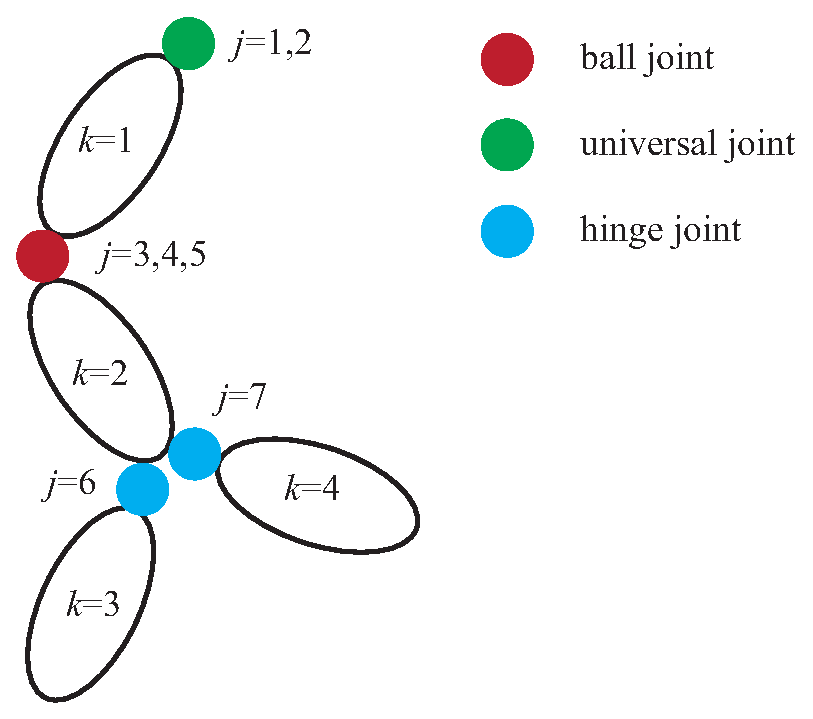
\includegraphics[width=2.1in]{example1.eps}
\end{center}
\caption{An articulated system.}
 \vspace{-20pt}
\label{fig:example1}
\end{wrapfigure}

Now, consider a multibody system with $m$ rigid links. Before we look
at its angular velocity, let us first define a few notations.
\begin{itemize}
\item $s(k)$ returns the index set of DOFs in link $k$, and $s(1, k)$
  returns the index set of DOFs in the chain of links from the root to
  the link $k$. For example in Figure \ref{fig:example1}, $s(2) = \{3, 4, 5\}$, $s(1, 4) = \{1, 2, 3,
    4, 5, 7\}$.
\item $p(k)$ returns the index of the parent link of link $k$. For
  example, $p(4) = 2$.
\item $l(j)$ returns the link index where DOF $j$ resides. For
  example, $l(5) = 2$.
\item $R^0_k$ is the chain of rotational transformations from the
  world frame to the local frame of the link $k$.
\end{itemize}

The angular velocity of link $k$ viewed in the world frame is then
\begin{eqnarray}
[\omega_k] & = & \dot{(R^0_{p(k)}R_k)} (R^0_{p(k)}R_k)^T = \sum_{j \in s(1,p(k))}
\frac{\partial R^0_{p(k)}}{\partial q_j} R_k R_k^T (R^0_{p(k)})^T
\dot{q}_j + \sum_{j \in s(k)} R^0_{p(k)} \frac{\partial R_k}{\partial q_j} R_k^T
(R^0_{p(k)})^T \dot{q}_j  \nonumber \\
& = & \sum_{j \in s(1,k)} (R^0_{p(l(j))} [\vc{u}_{l(j)j}] (R^0_{p(l(j))})^T) \dot{q}_j, \;\;\;\mathrm{where}\;\;
[\vc{u}_{l(j)j}] = \frac{\partial R_{l(j)}}{\partial q_j} R_{l(j)}^T
\end{eqnarray}
\ignorethis{
\begin{eqnarray}
[\omega_k] & = & \dot{(R^0_{k-1}R_k)} (R^0_{k-1}R_k)^T = \sum_j
\frac{\partial R^0_{k-1}}{\partial q_j} R_k R_k^T (R^0_{k-1})^T
\dot{q}_j + \sum_j R^0_{k-1} \frac{\partial R_k}{\partial q_j} R_k^T
(R^0_{k-1})^T \dot{q}_j  \nonumber \\
& = & \sum_j ([\vc{s}_j] +R^0_{k-1} [\vc{t}_j] (R^0_{k-1})^T) \dot{q}_j, \;\;\;\mathrm{where}\;\;
\vc{s}_j = \frac{\partial R^0_{k-1}}{\partial q_j} (R^0_{k-1})^T, \;\;
\vc{t}_j = \frac{\partial R_k}{\partial q_j} R_k^T
\end{eqnarray}
}

Using the property of skew symmetric matrix, $[R \vc{u}] = R [\vc{u}]
R^T$, we can express the angular velocity in the vector form as
\begin{equation}
\label{eqn:angular_velocity}
\omega_k = (\vc{u}_{11} \cdots R^0_{p(l(j))} \vc{u}_{l(j)j} \cdots \vc{0}) \dot{\vc{q}} = J_{\omega k} \dot{\vc{q}}
\end{equation}
where $j$ is in the set of $s(1,k)$, and $J_{\omega k}$ is a $3 \times
n$ matrix. Note that the zero columns in $J_{\omega k}$ correspond to
DOFs that are not in the chain of transformations from the root to the
link $k$. Let us look at a couple of examples using the articulated
rigid body system in Figure \ref{fig:example1}:
\begin{eqnarray}
\omega_1 &=& (\vc{u}_{11} \;\; \vc{u}_{12} \;\; \vc{0}
\;\;\vc{0}\;\;\vc{0}\;\;\vc{0}\;\;\vc{0}) \dot{\vc{q}}  \nonumber \\
\omega_4 &=& (\vc{u}_{11} \;\; \vc{u}_{12} \;\; R^0_1\vc{u}_{23} \;\;
R^0_1\vc{u}_{24} \;\;  R^0_1\vc{u}_{25} \;\; \vc{0} \;\;
R^0_2 \vc{u}_{47}) \dot{\vc{q}} \nonumber
\end{eqnarray}
where $\vc{u}$, $R\vc{u}$, and $\vc{0}$ are all $3\times 1$
vectors. Depending on the representation of the rotation matrix,
$\vc{u}$ can assume different values. For example, if the joint
between link $1$ and link $2$ in Figure \ref{fig:example1} is
represented as three Euler rotations, $R^{(x)}$, $R^{(y)}$, and
$R^{(z)}$, we have $\vc{u}_{23} = (1\;\; 0 \;\; 0)^T$, $\vc{u}_{24} =
R^{(x)} (0\;\;1\;\;0)^T$, and $\vc{u}_{25} = R^{(x)}R^{(y)}
(0\;\;0\;\;1)^T$. If the joint is represented as a quaternion or an
exponential map, $\vc{u}$ do not have a simple symbolic form.

\ignorethis{
\begin{equation}
\label{eqn:angular_velocity}
\omega_k = (\vc{s}_1 \cdots \vc{s}_{np} \; R^0_{k-1} \vc{t}_1 \cdots
R^0_{k-1} \vc{t}_{nk}\; \vc{0} \cdots \vc{0}) \dot{\vc{q}} = J_{\omega k} \dot{\vc{q}}
\end{equation}
where $np$ is the number of DOFs in the parent chain and $nk$ is the
number of DOFs in the link $k$. 
}

Similarly, the linear velocity of the center of mass of the link $k$
can be expressed in terms of the generalized velocity: 
\begin{equation}
\vc{v}_k = J_{vk} \dot{\vc{q}}, \;\;\;\mathrm{where}\;\; J_{vk} = \frac{\partial T^0_k
  \vc{c}_k}{\partial \vc{q}}.
\end{equation}
where the chain of transformations from the world frame to the local
frame of link $k$ is denoted as $T^0_k$. Note that $T^0_k$ is
different from $R^0_k$ in that $T^0_k$ includes the translational
transformations. $\vc{c}$ denotes the center of mass of link $k$ in
its local frame.

We can concatenate all $2m$  Jacobian matrices into a single Jacobian
that relates the generalized velocity to the Cartesian velocity of each
link:
\begin{equation}
\left[
\begin{array}{c}
\vc{v} \\
\omega \\
\end{array}
\right] =
\left[
\begin{array}{c}
\vc{v}_1 \\
\vdots \\
\vc{v}_m \\
\omega_1 \\
\vdots \\
\omega_m
\end{array}
\right] = 
\left[
\begin{array}{c}
J_{v1} \\
\vdots \\
J_{vm} \\
J_{\omega 1} \\
\vdots \\
J_{\omega m}
\end{array}
\right] 
\left[
\begin{array}{c}
\dot{q}_1\\
\vdots \\
\dot{q}_n
\end{array}
\right]  = J \dot{\vc{q}}
\end{equation}

Typically, the Jacobian $J$ is full column rank because the
number of DOFs in the maximal representation is more than that in the
generalized representation, i.e $6m > n$. To compute $\dot{\vc{q}}$ from $(\vc{v}, \omega)$, we
will end up solving a over-constrained linear system. We can use
pseudo inverse of $J$ to compute $\dot{\vc{q}}$:
\begin{equation}
 \dot{\vc{q}} = (J^TJ)^{-1}J^T
\left[
\begin{array}{c}
\vc{v} \\
\omega
\end{array}
\right]
 = J^+
\left[
\begin{array}{c}
\vc{v} \\
\omega
\end{array}
\right]
\end{equation}

Alternatively, we can rewrite the equation using the relative angular
velocity between a child and a parent link expressed in the local
frame of the parent, instead of using angular velocity of each link
expressed in the world frame.
\begin{equation}
\hat{\omega}_k = (R^0_{p(k)})^T(\omega_k - \omega_{p(k)}) = (\vc{0} \cdots \vc{0} \;\; \vc{u}_{l(j)j} \;\; \vc{0}
\cdots \vc{0}) \dot{\vc{q}} = \hat{J}_{\omega k} \dot{\vc{q}} 
\end{equation}
where $j$ is in the set of $s(k)$. Comparing the above equation with Equation \ref{eqn:angular_velocity},
the angular part of Jacobian, $\hat{J}_\omega$, is usually more sparse
that $J_\omega$.

\ignorethis{
\begin{equation}
\hat{\omega}_k = (\vc{0} \cdots \vc{0} \;\vc{t}_1 \cdots \vc{t}_{nk}\;
\vc{0} \cdots \vc{0}) \dot{\vc{q}} = \hat{J}_{\omega k} \dot{\vc{q}} 
\end{equation}
}

\subsection{Force conversion}
The relation between the Cartesian force and the generalized force can
be found in Equation \ref{eqn:virtual_work}:
\begin{equation}
\label{eqn:force_conversion}
\vc{Q} = \sum_i J_{vi}^T \vc{f}_i + \sum_k J_{\omega k}^T \tau_k = 
\left[
\begin{array}{cc}
J_{v}^T & J_\omega^T
\end{array}
\right]
\left[
\begin{array}{c}
\vc{f} \\
\tau
\end{array}
\right] 
, \;\;\;\mathrm{where}\;\;
J_{vi} = \frac{\partial \vc{r}_i}{\partial \vc{q}}
\end{equation}
where $\vc{r}_i$ is the point of application of the Cartesian force
$\vc{f}_i$ expressed in the world frame. Body torque $\tau_k$ is the torque
applied on link $k$. 

Sometimes it is more convenient to express \emph{joint torques} in the
local frame of the parent link, rather than \emph{body torques} in the
world frame. For example, the joint torque between link $p(k)$ and
link $k$ can be computed as $\hat{\tau}_{p(k)} = (R^0_{p(k)})^T(\tau_{p(k)} -
\tau_k)$. Equation \ref{eqn:force_conversion} is then modified to:
\begin{equation}
\vc{Q} = \left[
\begin{array}{cc}
J_{v}^T & J_\omega^T
\end{array}
\right]
\left[
\begin{array}{c}
\vc{f} \\
\tau
\end{array}
\right] 
 = \left[
\begin{array}{cc}
J_{v}^T & J_\omega^T
\end{array}
\right]
\left[
\begin{array}{c}
\vc{f} \\
D 
\left[
\begin{array}{c}
R^0_{p(1)} \hat{\tau}_1 \\
\vdots \\
R^0_{p(m)}) \hat{\tau}_m
\end{array}
\right]
\end{array}
\right] =
\left[
\begin{array}{cc}
J_{v}^T & \hat{J}_\omega^T
\end{array}
\right]
\left[
\begin{array}{c}
\vc{f} \\
\hat{\tau}
\end{array}
\right]  
\end{equation}
where matrix $D$ encodes the relation between body torques and joint
torques. For example, matrix $D$ for the system in Figure \ref{fig:example1} looks
like:
\begin{equation}
D =
\left[
\begin{array}{cccc}
\vc{I}_{3\time 3}  & -\vc{I}_{3\time 3} & \vc{0} & \vc{0}\\
\vc{0} & \vc{I}_{3\time 3}  & -\vc{I}_{3\time 3} & -\vc{I}_{3\time 3}\\
\vc{0} & \vc{0} & \vc{I}_{3\time 3}  & \vc{0}\\
\vc{0} & \vc{0} & \vc{0} & \vc{I}_{3\time 3}\\
\end{array}
\right]  
\end{equation}


\section{Recursive Inverse and Forward Dynamics}